% Generated by Sphinx.
\def\sphinxdocclass{report}
\documentclass[letterpaper,10pt,dvipdfmx,openany]{sphinxmanual}
\usepackage[utf8]{inputenc}
\DeclareUnicodeCharacter{00A0}{\nobreakspace}
\usepackage{cmap}
\usepackage[T1]{fontenc}
\usepackage[english]{babel}
\usepackage{times}
\usepackage[Sonny]{fncychap}
\usepackage{longtable}
\usepackage{sphinx}
\usepackage{multirow}


\title{Shiftk Documentation}
\date{January 27, 2017}
\release{0.1}
\author{kawamura}
\newcommand{\sphinxlogo}{}
\renewcommand{\releasename}{Release}
\makeindex

\makeatletter
\def\PYG@reset{\let\PYG@it=\relax \let\PYG@bf=\relax%
    \let\PYG@ul=\relax \let\PYG@tc=\relax%
    \let\PYG@bc=\relax \let\PYG@ff=\relax}
\def\PYG@tok#1{\csname PYG@tok@#1\endcsname}
\def\PYG@toks#1+{\ifx\relax#1\empty\else%
    \PYG@tok{#1}\expandafter\PYG@toks\fi}
\def\PYG@do#1{\PYG@bc{\PYG@tc{\PYG@ul{%
    \PYG@it{\PYG@bf{\PYG@ff{#1}}}}}}}
\def\PYG#1#2{\PYG@reset\PYG@toks#1+\relax+\PYG@do{#2}}

\expandafter\def\csname PYG@tok@gd\endcsname{\def\PYG@tc##1{\textcolor[rgb]{0.63,0.00,0.00}{##1}}}
\expandafter\def\csname PYG@tok@gu\endcsname{\let\PYG@bf=\textbf\def\PYG@tc##1{\textcolor[rgb]{0.50,0.00,0.50}{##1}}}
\expandafter\def\csname PYG@tok@gt\endcsname{\def\PYG@tc##1{\textcolor[rgb]{0.00,0.27,0.87}{##1}}}
\expandafter\def\csname PYG@tok@gs\endcsname{\let\PYG@bf=\textbf}
\expandafter\def\csname PYG@tok@gr\endcsname{\def\PYG@tc##1{\textcolor[rgb]{1.00,0.00,0.00}{##1}}}
\expandafter\def\csname PYG@tok@cm\endcsname{\let\PYG@it=\textit\def\PYG@tc##1{\textcolor[rgb]{0.25,0.50,0.56}{##1}}}
\expandafter\def\csname PYG@tok@vg\endcsname{\def\PYG@tc##1{\textcolor[rgb]{0.73,0.38,0.84}{##1}}}
\expandafter\def\csname PYG@tok@m\endcsname{\def\PYG@tc##1{\textcolor[rgb]{0.13,0.50,0.31}{##1}}}
\expandafter\def\csname PYG@tok@mh\endcsname{\def\PYG@tc##1{\textcolor[rgb]{0.13,0.50,0.31}{##1}}}
\expandafter\def\csname PYG@tok@cs\endcsname{\def\PYG@tc##1{\textcolor[rgb]{0.25,0.50,0.56}{##1}}\def\PYG@bc##1{\setlength{\fboxsep}{0pt}\colorbox[rgb]{1.00,0.94,0.94}{\strut ##1}}}
\expandafter\def\csname PYG@tok@ge\endcsname{\let\PYG@it=\textit}
\expandafter\def\csname PYG@tok@vc\endcsname{\def\PYG@tc##1{\textcolor[rgb]{0.73,0.38,0.84}{##1}}}
\expandafter\def\csname PYG@tok@il\endcsname{\def\PYG@tc##1{\textcolor[rgb]{0.13,0.50,0.31}{##1}}}
\expandafter\def\csname PYG@tok@go\endcsname{\def\PYG@tc##1{\textcolor[rgb]{0.20,0.20,0.20}{##1}}}
\expandafter\def\csname PYG@tok@cp\endcsname{\def\PYG@tc##1{\textcolor[rgb]{0.00,0.44,0.13}{##1}}}
\expandafter\def\csname PYG@tok@gi\endcsname{\def\PYG@tc##1{\textcolor[rgb]{0.00,0.63,0.00}{##1}}}
\expandafter\def\csname PYG@tok@gh\endcsname{\let\PYG@bf=\textbf\def\PYG@tc##1{\textcolor[rgb]{0.00,0.00,0.50}{##1}}}
\expandafter\def\csname PYG@tok@ni\endcsname{\let\PYG@bf=\textbf\def\PYG@tc##1{\textcolor[rgb]{0.84,0.33,0.22}{##1}}}
\expandafter\def\csname PYG@tok@nl\endcsname{\let\PYG@bf=\textbf\def\PYG@tc##1{\textcolor[rgb]{0.00,0.13,0.44}{##1}}}
\expandafter\def\csname PYG@tok@nn\endcsname{\let\PYG@bf=\textbf\def\PYG@tc##1{\textcolor[rgb]{0.05,0.52,0.71}{##1}}}
\expandafter\def\csname PYG@tok@no\endcsname{\def\PYG@tc##1{\textcolor[rgb]{0.38,0.68,0.84}{##1}}}
\expandafter\def\csname PYG@tok@na\endcsname{\def\PYG@tc##1{\textcolor[rgb]{0.25,0.44,0.63}{##1}}}
\expandafter\def\csname PYG@tok@nb\endcsname{\def\PYG@tc##1{\textcolor[rgb]{0.00,0.44,0.13}{##1}}}
\expandafter\def\csname PYG@tok@nc\endcsname{\let\PYG@bf=\textbf\def\PYG@tc##1{\textcolor[rgb]{0.05,0.52,0.71}{##1}}}
\expandafter\def\csname PYG@tok@nd\endcsname{\let\PYG@bf=\textbf\def\PYG@tc##1{\textcolor[rgb]{0.33,0.33,0.33}{##1}}}
\expandafter\def\csname PYG@tok@ne\endcsname{\def\PYG@tc##1{\textcolor[rgb]{0.00,0.44,0.13}{##1}}}
\expandafter\def\csname PYG@tok@nf\endcsname{\def\PYG@tc##1{\textcolor[rgb]{0.02,0.16,0.49}{##1}}}
\expandafter\def\csname PYG@tok@si\endcsname{\let\PYG@it=\textit\def\PYG@tc##1{\textcolor[rgb]{0.44,0.63,0.82}{##1}}}
\expandafter\def\csname PYG@tok@s2\endcsname{\def\PYG@tc##1{\textcolor[rgb]{0.25,0.44,0.63}{##1}}}
\expandafter\def\csname PYG@tok@vi\endcsname{\def\PYG@tc##1{\textcolor[rgb]{0.73,0.38,0.84}{##1}}}
\expandafter\def\csname PYG@tok@nt\endcsname{\let\PYG@bf=\textbf\def\PYG@tc##1{\textcolor[rgb]{0.02,0.16,0.45}{##1}}}
\expandafter\def\csname PYG@tok@nv\endcsname{\def\PYG@tc##1{\textcolor[rgb]{0.73,0.38,0.84}{##1}}}
\expandafter\def\csname PYG@tok@s1\endcsname{\def\PYG@tc##1{\textcolor[rgb]{0.25,0.44,0.63}{##1}}}
\expandafter\def\csname PYG@tok@gp\endcsname{\let\PYG@bf=\textbf\def\PYG@tc##1{\textcolor[rgb]{0.78,0.36,0.04}{##1}}}
\expandafter\def\csname PYG@tok@sh\endcsname{\def\PYG@tc##1{\textcolor[rgb]{0.25,0.44,0.63}{##1}}}
\expandafter\def\csname PYG@tok@ow\endcsname{\let\PYG@bf=\textbf\def\PYG@tc##1{\textcolor[rgb]{0.00,0.44,0.13}{##1}}}
\expandafter\def\csname PYG@tok@sx\endcsname{\def\PYG@tc##1{\textcolor[rgb]{0.78,0.36,0.04}{##1}}}
\expandafter\def\csname PYG@tok@bp\endcsname{\def\PYG@tc##1{\textcolor[rgb]{0.00,0.44,0.13}{##1}}}
\expandafter\def\csname PYG@tok@c1\endcsname{\let\PYG@it=\textit\def\PYG@tc##1{\textcolor[rgb]{0.25,0.50,0.56}{##1}}}
\expandafter\def\csname PYG@tok@kc\endcsname{\let\PYG@bf=\textbf\def\PYG@tc##1{\textcolor[rgb]{0.00,0.44,0.13}{##1}}}
\expandafter\def\csname PYG@tok@c\endcsname{\let\PYG@it=\textit\def\PYG@tc##1{\textcolor[rgb]{0.25,0.50,0.56}{##1}}}
\expandafter\def\csname PYG@tok@mf\endcsname{\def\PYG@tc##1{\textcolor[rgb]{0.13,0.50,0.31}{##1}}}
\expandafter\def\csname PYG@tok@err\endcsname{\def\PYG@bc##1{\setlength{\fboxsep}{0pt}\fcolorbox[rgb]{1.00,0.00,0.00}{1,1,1}{\strut ##1}}}
\expandafter\def\csname PYG@tok@kd\endcsname{\let\PYG@bf=\textbf\def\PYG@tc##1{\textcolor[rgb]{0.00,0.44,0.13}{##1}}}
\expandafter\def\csname PYG@tok@ss\endcsname{\def\PYG@tc##1{\textcolor[rgb]{0.32,0.47,0.09}{##1}}}
\expandafter\def\csname PYG@tok@sr\endcsname{\def\PYG@tc##1{\textcolor[rgb]{0.14,0.33,0.53}{##1}}}
\expandafter\def\csname PYG@tok@mo\endcsname{\def\PYG@tc##1{\textcolor[rgb]{0.13,0.50,0.31}{##1}}}
\expandafter\def\csname PYG@tok@mi\endcsname{\def\PYG@tc##1{\textcolor[rgb]{0.13,0.50,0.31}{##1}}}
\expandafter\def\csname PYG@tok@kn\endcsname{\let\PYG@bf=\textbf\def\PYG@tc##1{\textcolor[rgb]{0.00,0.44,0.13}{##1}}}
\expandafter\def\csname PYG@tok@o\endcsname{\def\PYG@tc##1{\textcolor[rgb]{0.40,0.40,0.40}{##1}}}
\expandafter\def\csname PYG@tok@kr\endcsname{\let\PYG@bf=\textbf\def\PYG@tc##1{\textcolor[rgb]{0.00,0.44,0.13}{##1}}}
\expandafter\def\csname PYG@tok@s\endcsname{\def\PYG@tc##1{\textcolor[rgb]{0.25,0.44,0.63}{##1}}}
\expandafter\def\csname PYG@tok@kp\endcsname{\def\PYG@tc##1{\textcolor[rgb]{0.00,0.44,0.13}{##1}}}
\expandafter\def\csname PYG@tok@w\endcsname{\def\PYG@tc##1{\textcolor[rgb]{0.73,0.73,0.73}{##1}}}
\expandafter\def\csname PYG@tok@kt\endcsname{\def\PYG@tc##1{\textcolor[rgb]{0.56,0.13,0.00}{##1}}}
\expandafter\def\csname PYG@tok@sc\endcsname{\def\PYG@tc##1{\textcolor[rgb]{0.25,0.44,0.63}{##1}}}
\expandafter\def\csname PYG@tok@sb\endcsname{\def\PYG@tc##1{\textcolor[rgb]{0.25,0.44,0.63}{##1}}}
\expandafter\def\csname PYG@tok@k\endcsname{\let\PYG@bf=\textbf\def\PYG@tc##1{\textcolor[rgb]{0.00,0.44,0.13}{##1}}}
\expandafter\def\csname PYG@tok@se\endcsname{\let\PYG@bf=\textbf\def\PYG@tc##1{\textcolor[rgb]{0.25,0.44,0.63}{##1}}}
\expandafter\def\csname PYG@tok@sd\endcsname{\let\PYG@it=\textit\def\PYG@tc##1{\textcolor[rgb]{0.25,0.44,0.63}{##1}}}

\def\PYGZbs{\char`\\}
\def\PYGZus{\char`\_}
\def\PYGZob{\char`\{}
\def\PYGZcb{\char`\}}
\def\PYGZca{\char`\^}
\def\PYGZam{\char`\&}
\def\PYGZlt{\char`\<}
\def\PYGZgt{\char`\>}
\def\PYGZsh{\char`\#}
\def\PYGZpc{\char`\%}
\def\PYGZdl{\char`\$}
\def\PYGZhy{\char`\-}
\def\PYGZsq{\char`\'}
\def\PYGZdq{\char`\"}
\def\PYGZti{\char`\~}
% for compatibility with earlier versions
\def\PYGZat{@}
\def\PYGZlb{[}
\def\PYGZrb{]}
\makeatother

\begin{document}

\maketitle
\tableofcontents
\phantomsection\label{index::doc}



\chapter{Overview}
\label{shiftk_overview_en:overview}\label{shiftk_overview_en:welcome-to-sample-program-s-documentation}\label{shiftk_overview_en::doc}
This is document for the sample program which uses
K \(\omega\) library in the ISSP Math Library;
this program computes the Green's function with \(K(\omega)\).
For the details of K \(\omega\) library, See
``\(K(\omega)\) manual'' in this package.


\section{Calculation in this program}
\label{shiftk_overview_en:calculation-in-this-program}
This program compute the Green's function
\begin{gather}
\begin{split}\begin{align}
G_{i}(z) =
\langle i | (z-{\hat H})^{-1}| i \rangle
\equiv
{\boldsymbol \varphi}_i^{*} \cdot (z-{\hat H})^{-1} {\boldsymbol \varphi}_i,
\end{align}\end{split}\notag
\end{gather}
where \(| i \rangle\) is a wavefunction,
\({\cal H}\) is the Hamiltonian, and
\(z\) is a complex frequency.
\begin{description}
\item[{\({\cal H}\) in the above equation is obtained by either the}] \leavevmode
following two ways:

\end{description}
\begin{itemize}
\item {} 
Input \({\cal H}\) as a file with the MatrixMarket format

\item {} 
Construct \({\cal H}\) as a Hamiltonian of the
Heisenberg model in this program.

\end{itemize}

In the computation of the Green's function,
we use either the following two method according to the type
of \({\hat H}\) (a real- or a complex- number).
\begin{itemize}
\item {} 
\({\hat H}\) of real numbers : Shifted Bi-Conjugate Gradient(BiCG) method

\item {} 
\({\hat H}\) of complex numbers : Shifted Conjugate Orthogonal Conjugate Gradient(COCG) method

\end{itemize}


\chapter{License}
\label{shiftk_copy_en::doc}\label{shiftk_copy_en:license}
\emph{© 2016- The University of Tokyo. All rights reserved.}

\begin{DUlineblock}{0em}
\item[] This software is developed under the support of
\item[] ``\emph{Project for advancement of software usability in materials science}'' by The
\item[] Institute for Solid State Physics, The University of Tokyo.
\item[] 
\item[] This library is free software; you can redistribute it and/or
\item[] modify it under the terms of the GNU Lesser General Public
\item[] License as published by the Free Software Foundation; either
\item[] version 2.1 of the License, or (at your option) any later version.
\item[] This library is distributed in the hope that it will be useful,
\item[] but WITHOUT ANY WARRANTY; without even the implied warranty of
\item[] MERCHANTABILITY or FITNESS FOR A PARTICULAR PURPOSE. See the GNU
\item[] Lesser General Public License for more details.
\item[] 
\item[] You should have received a copy of the GNU Lesser General Public
\item[] License along with this library; if not, write to the Free Software
\item[] Foundation, Inc., 59 Temple Place, Suite 330, Boston, MA 02111-1307 USA
\item[] 
\item[] For more details, See ‘COPYING.LESSER’ in the root directory of this library.
\end{DUlineblock}


\chapter{Prerequisite}
\label{shiftk_env_en::doc}\label{shiftk_env_en:prerequisite}\begin{itemize}
\item {} 
fortran compiler

\item {} 
K \(omega\) library

\item {} 
BLAS, LAPACK

\item {} 
MPI library (Optional)

\end{itemize}


\chapter{Overall procedure}
\label{shiftk_flow_en:overall-procedure}\label{shiftk_flow_en::doc}
This program performs simulation as follows (See Fig. \ref{shiftk_flow_en:calcflow} ):
\begin{enumerate}
\item {} 
Read a input file for the numerical condition.

\item {} 
(Optional) Read input files for the Hamiltonian and the right hand side vector.

\item {} 
(Optional) Read a file for the restart (\(\alpha\), \(\beta\), residual vectors)

\item {} 
(Bi)CG iteration with \(K\omega\) library

\item {} 
Output results (Green's function, residual vectors, \(\alpha\), \(\beta\))

\end{enumerate}
\begin{figure}[htbp]
\centering
\capstart

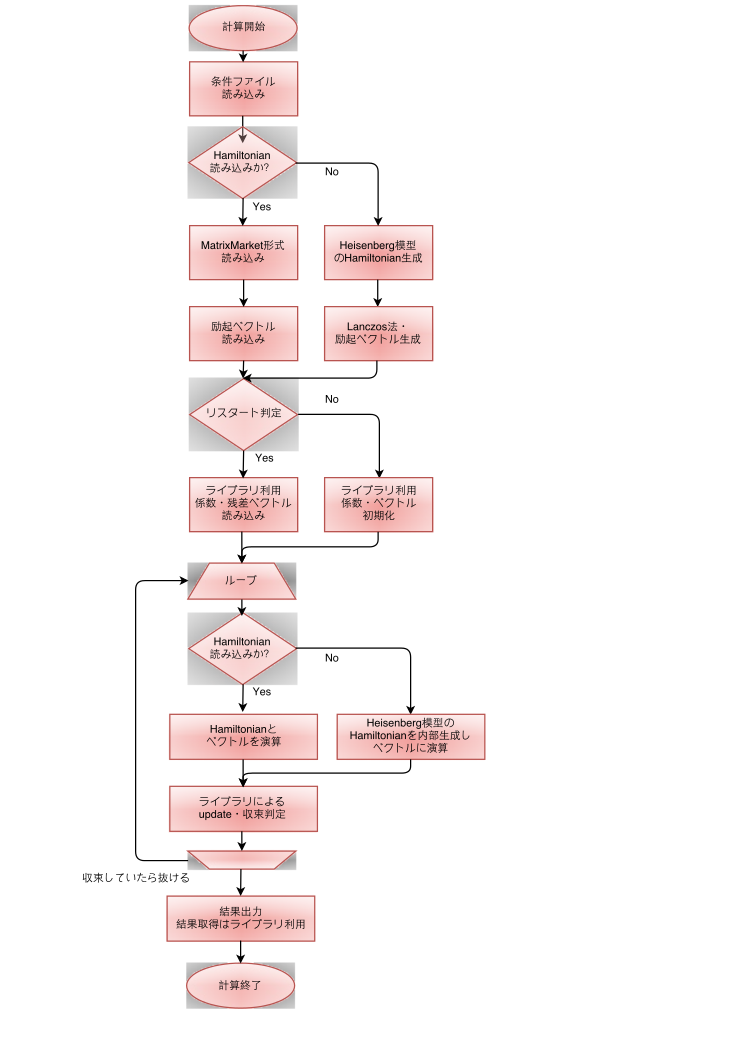
\includegraphics{flow.png}
\caption{Schematic flow of the calculation of this program.}\label{shiftk_flow_en:calcflow}\end{figure}

We introduce the detailed procedure as follows.
The format of each file is written in {\hyperref[shiftk_format_en:fileformat]{\emph{Format of files}}}.


\section{Calculation from scratch}
\label{shiftk_flow_en:calculation-from-scratch}

\subsection{Prepare input file}
\label{shiftk_flow_en:prepare-input-file}
In this input file, we specify the frequency grid,
the maximum number of iteration, etc.

A example of this input file is shown as follow.

\begin{Verbatim}[commandchars=\\\{\}]
\PYGZam{}filename
  inham = \PYGZdq{}\PYGZdq{}
  invec = \PYGZdq{}\PYGZdq{}
/
\PYGZam{}ham
nsite = 4
Jx = 1d0
Jy = 1d0
Jz = 1d0
Dz = 0d0
/
\PYGZam{}cg
  maxloops = 100
  convfactor = 6
/
\PYGZam{}dyn
  calctype = \PYGZdq{}normal\PYGZdq{}
  nomega = 100
  omegamin = (\PYGZhy{}2d0, 0.1d0)
  omegamax = ( 1d0, 0.1d0)
  outrestart = .TRUE.
/
\end{Verbatim}

where \code{InHam} is the file-name for the Hamiltonian in the MatrixMarket format,
\code{InVec} is the file-name of the right hand side vector,
\code{NOmega} is the number of frequencies where the dynamical Green's function
is computed.
\code{OmegaMin} is the lower limit of the frequency \(z\),
\code{OmegaMax} is the upper limit of the frequency \(z\).
These complex frequencies must be written as ``\code{(\{Real part\}, \{Imaginaly part\})}''.
The frequency grid is defined as
\begin{gather}
\begin{split}\begin{align}
\omega_n =  {\tt OmegaMin}
+ \frac{n-1}{{\tt NOmega}-1}({\tt OmegaMax} - {\tt OmegaMin}).
\end{align}\end{split}\notag
\end{gather}
\code{MaxLoops} is the maximum number of iterations.
For the details of this input file, see {\hyperref[shiftk_format_en:modpara]{\emph{``Namelist'' file}}}.
The string variable must be specified with two \code{'} or \code{"}.


\subsection{(Optional) Prepare input file for the Hamiltonian and RHS vector}
\label{shiftk_flow_en:optional-prepare-input-file-for-the-hamiltonian-and-rhs-vector}
Prepare input files for the Hamiltonian (MatrixMarket format)
and right hand side vector.

An example of the file of the right hand side vector
is shown as follows:

\begin{Verbatim}[commandchars=\\\{\}]
256
0.01    0.0
0.05    0.0
0.1     0.0
(continue ...)
\end{Verbatim}

Details of the file format is written in
{\hyperref[shiftk_format_en:ham]{\emph{``InHam'' file}}} and {\hyperref[shiftk_format_en:vec]{\emph{``InVec'' file}}}.


\subsection{Launch}
\label{shiftk_flow_en:launch}
Execute a program \code{ShiftK.out} with a namelist file \code{namelist.def}
as follows:

\begin{Verbatim}[commandchars=\\\{\}]
\PYG{n+nv}{\PYGZdl{} }ShiftK.out namelist.def
\end{Verbatim}


\subsection{Output}
\label{shiftk_flow_en:output}
The following files are generated in \code{output/} directory (this directory is
also generated by this program).

\begin{Verbatim}[commandchars=\\\{\}]
\PYG{n}{TriDiagComp}\PYG{o}{.}\PYG{n}{dat}\PYG{p}{,} \PYG{n}{ResVec}\PYG{o}{.}\PYG{n}{dat}\PYG{p}{,} \PYG{n}{dynamicalG}\PYG{o}{.}\PYG{n}{dat}
\end{Verbatim}

where
\code{TriDiagComp.dat} contains the parameters for the restart,
\code{ResVec.dat} contains the residual vector,
\code{dynamicalG.dat} contains the dynamical Green's function.
The format of these file is written in
{\hyperref[shiftk_format_en:revec]{\emph{Residual vector}}} - {\hyperref[shiftk_format_en:dynamicalg]{\emph{Dynamical Green's function}}}.


\section{Catch up}
\label{shiftk_flow_en:catch-up}
Compute the Green's function at the different frequency by using the information
of \code{output/TriDiagComp.dat} that are generated in the previous run.
This calculation does not require the matrix-vector product.


\subsection{Modify the namelist file}
\label{shiftk_flow_en:modify-the-namelist-file}
Change \code{calctype} parameter in the file \code{namelist.def}
from \code{"normal"} to \code{"recalc"}.
\code{OmegaMin}, \code{OmegaMax}, etc. can be modified.


\subsection{Launch}
\label{shiftk_flow_en:id1}
Execute a program \code{ShiftK.out} with a namelist file \code{namelist.def}
as follows:

\begin{Verbatim}[commandchars=\\\{\}]
\PYG{n+nv}{\PYGZdl{} }ShiftK.out namelist.def
\end{Verbatim}

The \code{output/dynamicalG.dat} will be overwritten.


\subsection{Output}
\label{shiftk_flow_en:id2}
The same output files as the previous section are generated.


\section{Restart}
\label{shiftk_flow_en:restart}
Compute the Green's function at the different frequency by using the information
of \code{output/TriDiagComp.dat} and \code{output/ResVec.dat}
that are generated in the previous run.


\subsection{Modify the namelist file}
\label{shiftk_flow_en:id3}
Change \code{calctype} parameter in the file \code{namelist.def}
from \code{"normal"} to \code{"restart"}.
\code{OmegaMin}, \code{OmegaMax}, etc. can be modified.
Parameters \code{InHam} ,  \code{InVec}, and the files of the Hamiltonian
and RHS vector can not be modified.


\subsection{Launch}
\label{shiftk_flow_en:id4}
Execute a program \code{ShiftK.out} with a namelist file \code{namelist.def}
as follows:

\begin{Verbatim}[commandchars=\\\{\}]
\PYG{n+nv}{\PYGZdl{} }ShiftK.out namelist.def
\end{Verbatim}

The \code{output/dynamicalG.dat} will be overwritten.


\subsection{Output}
\label{shiftk_flow_en:id5}
The following files are generated (or are overwritten) in \code{output/} directory.

\begin{Verbatim}[commandchars=\\\{\}]
\PYG{n}{TriDiagComp}\PYG{o}{.}\PYG{n}{dat}\PYG{p}{,} \PYG{n}{ResVec}\PYG{o}{.}\PYG{n}{dat}\PYG{p}{,} \PYG{n}{dynamicalG}\PYG{o}{.}\PYG{n}{dat}
\end{Verbatim}

where
\code{TriDiagComp.dat} contains the parameters for the restart,
\code{ResVec.dat} contains the residual vector,
\code{dynamicalG.dat} contains the dynamical Green's function.
The format of these file is written in
{\hyperref[shiftk_format_en:revec]{\emph{Residual vector}}} - {\hyperref[shiftk_format_en:dynamicalg]{\emph{Dynamical Green's function}}}.


\chapter{Format of files}
\label{shiftk_format_en:format-of-files}\label{shiftk_format_en::doc}\label{shiftk_format_en:fileformat}

\section{Input files}
\label{shiftk_format_en:input-files}

\subsection{``Namelist'' file}
\label{shiftk_format_en:modpara}\label{shiftk_format_en:namelist-file}
This file has four namelist (\code{filename}, \code{ham}, \code{cg}, \code{dyn}).
For the details of the namelist of fortran, see some books and Web page for fortran.

\begin{Verbatim}[commandchars=\\\{\}]
\PYGZam{}filename
  inham = \PYGZdq{}\PYGZdq{}
  invec = \PYGZdq{}\PYGZdq{}
/
\PYGZam{}ham
nsite = 4
Jx = 1d0
Jy = 1d0
Jz = 1d0
Dz = 0d0
/
\PYGZam{}cg
  maxloops = 100
  convfactor = 6
/
\PYGZam{}dyn
  calctype = \PYGZdq{}normal\PYGZdq{}
  nomega = 100
  omegamin = (\PYGZhy{}2d0, 0.1d0)
  omegamax = ( 1d0, 0.1d0)
  outrestart = .TRUE.
/
\end{Verbatim}

In the namelist \emph{``filename''{}`}, we specify the file names of the
Hamiltonian and the RHS vector.
\begin{itemize}
\item {} 
\code{InHam}

\textbf{Type :} string (default: \code{""})

\textbf{Description :}
The name of the file for the Hamiltonian in the MatrixMarket format
(full path or relative path).
If this parameter is not specified,
the Hamiltonian of the 1D spin chain is generated
with the parameters in \code{ham} namelist.

\item {} 
\code{InVec}

\textbf{Type :} string (default: \code{""})

\textbf{Description :}
The name of the file for the right hand side vector.
If this parameter is not specified,
the RHS vector is generated as follows:
First the ground-state vector is computed.
Then RHS vector is calculated by operating
\({\hat S}_{1 z}\) (\(z\) component of the spin at site 1)
to the ground-state vector.
Therefore, we assume the computed system is
the one-dimensional spin chain.

\end{itemize}
\begin{description}
\item[{\code{"ham"} namelist is read only when}] \leavevmode
\code{InHam} is not specified.
The parameters in this namelist are used to generate
the Hamiltonian of the one-dimensional spin chain (See Fig. \ref{shiftk_format_en:spin})

\end{description}
\begin{gather}
\begin{split}\begin{align}
  {\hat H} = \sum_{i}
  \left(
  \begin{matrix}
    {\hat S}_{i x} & {\hat S}_{i y} & {\hat S}_{i z}
  \end{matrix}
  \right)
  \left(
  \begin{matrix}
    J_x & D_z & 0 \\
    -D_z & J_y & 0 \\
    0 & 0 & J_z
  \end{matrix}
  \right)
  \left(
  \begin{matrix}
    {\hat S}_{i+1 x} \ {\hat S}_{i+1 y} \ {\hat S}_{i+1 z}
  \end{matrix}
  \right).
  \end{align}\end{split}\notag
\end{gather}\begin{figure}[htbp]
\centering
\capstart

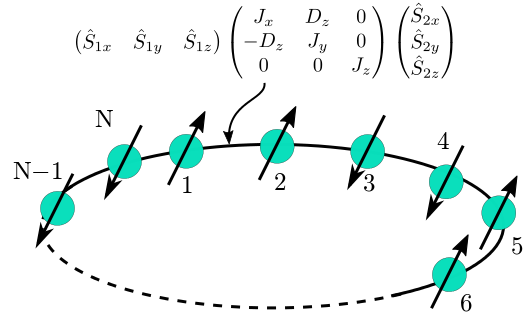
\includegraphics{spin.png}
\caption{Schematic picture of the one-dimensional spin chain.}\label{shiftk_format_en:spin}\end{figure}
\begin{itemize}
\item {} 
\code{nsite}

\textbf{Type :} int (default: \code{4})

\textbf{Description :}
The number of sites in the 1D spin chain model.

\item {} 
\code{Jx}

\textbf{Type :} double (default: \code{1.0})

\textbf{Description :} \(J_x\) for the Heisenberg model.

\item {} 
\code{Jy}

\textbf{Type :} double (default: \code{1.0})

\textbf{Description :} \(J_y\) for the Heisenberg model.

\item {} 
\code{Jz}

\textbf{Type :} double (default: \code{1.0})

\textbf{Description :} \(J_z\) for the Heisenberg model.

\item {} 
\code{Dz}

\textbf{Type :} double (default: \code{0.0})

\textbf{Description :}
The parameter of the Dzyaloshinskii-Moriya interaction (\(D_z\)).

\end{itemize}

\code{cg} namelist has parameters
for specifying the numerical condition for the
(Bi)Conjugate-gradient method.
\begin{itemize}
\item {} 
\code{MaxLoops}

\textbf{Type :} int (default: the dimension of the Hamiltonian)

\textbf{Description :} The maximum number of iterations.

\item {} 
\code{Convfactor}

\textbf{Type :} int (default: \code{8})

\textbf{Description :} Convergence threshold.
If the 2-norm of the residual vector becomes smaller than
\(10^{-{\tt Convfactor}}\), the calculation finishes.

\end{itemize}

\code{dyn} has the parameters for the computation of the spectrum.
\begin{itemize}
\item {} 
\code{OmegaMin}

\textbf{Type :} Complex (default: If \code{invec} is not specified,
the real part of it becomes the smallest eigenvalue,
and the imaginary part of it becomes \(\times0.01\) times
the difference between the largest- and the smallest- eigenvalue.
If \code{invec} is specified, the default value becomes \code{(0.0, 0.01)})

\textbf{Description :} The smallest frequency.

\item {} 
\code{OmegaMax}

\textbf{Type :} Complex (default: If \code{invec} is not specified,
the real part of it becomes the largest eigenvalue,
and the imaginary part of it becomes \(\times0.01\) times
the difference between the largest- and the smallest- eigenvalue.
If \code{invec} is specified, the default value becomes \code{(1.0, 0.01)})

\textbf{Description :} The largest frequency.

\item {} 
\code{NOmega}

\textbf{Type :} int (default: \code{10})

\textbf{Description :} The number of frequencies.

\item {} 
\code{outrestart}

\textbf{Type :} Logical (default: \code{.FALSE.})

\textbf{Description :}
Whether data for restart will be written (\code{.TRUE.}) or not (\code{.FALSE.}).

\item {} 
\code{calctype}

\textbf{Type :}
String.  Choose from \code{"normal"}, \code{"recalc"}, \code{"restart"}.
(default: \code{"normal"})

\textbf{Description :}
\code{"normal"} for computing with the Krylov subspace from scratch.
\code{"recalc"} for computing with the Krylov subspace
generated in the previous calculation.
In this case, the matrix-vector product is not performed.
The convergence is not guaranteed.
\code{"restart"} for restarting the calculation from the
previous run.
In this case, the calculation continues until
the convergence is achieved or the number of iteration becomes \code{MaxLoops}.

\end{itemize}


\subsection{``InHam'' file}
\label{shiftk_format_en:ham}\label{shiftk_format_en:inham-file}
The Hamiltonian is written in the MatrixMarket format.

Example of the ``InHam'' file:

\begin{Verbatim}[commandchars=\\\{\}]
\PYGZpc{}\PYGZpc{}MatrixMarket matrix coordinate complex hermitian
16 16 20
1 1 1.000000 0.000000
3 2 0.500000 0.000000
5 3 0.500000 0.000000
6 4 0.500000 0.000000
6 6 \PYGZhy{}1.000000 0.000000
7 6 0.500000 0.000000
9 2 0.500000 0.000000
9 5 0.500000 0.000000
10 6 0.500000 0.000000
11 4 0.500000 0.000000
11 7 0.500000 0.000000
11 10 0.500000 0.000000
11 11 \PYGZhy{}1.000000 0.000000
12 8 0.500000 0.000000
13 6 0.500000 0.000000
13 11 0.500000 0.000000
14 12 0.500000 0.000000
15 8 0.500000 0.000000
15 14 0.500000 0.000000
16 16 1.000000 0.000000
\end{Verbatim}
\begin{description}
\item[{First row:}] \leavevmode
Arbitrary string (such as comment).

\item[{Second row:}] \leavevmode
The number of rows, columns, and non-zero elements
(in \textbf{the lower triangle part}).

\item[{Third row - End:}] \leavevmode
The row- and the column- index, and
the real- and imaginary- part of the non-zero element
(in \textbf{the lower triangle part}).

\end{description}


\subsection{``InVec'' file}
\label{shiftk_format_en:vec}\label{shiftk_format_en:invec-file}
Right hand side vector is contained.

Example of the ``InVec'' file:

\begin{Verbatim}[commandchars=\\\{\}]
8192
0.02 0.01
0.02 0.001
(continue...)
\end{Verbatim}
\begin{itemize}
\item {} 
First row: {[} int01 {]}

\textbf{Type :} int

\textbf{Description :}
The dimension of the Hilbert space.
It must be the same as the dimension of the Hamiltonian.

\item {} 
Second row - End:
{[} double01 {]} {[} double02 {]}

\textbf{Type :} double

\textbf{Description :} The element of the RHS vector.
{[} double01 {]} is the real part,
and {[} double02 {]} is the imaginary part.

\end{itemize}


\subsection{Coefficients for restart}
\label{shiftk_format_en:recoeff}\label{shiftk_format_en:coefficients-for-restart}
The coefficient \(\alpha\) and \(\beta\)
are contained.

The name of the generated file is \code{TriDiagComp.dat}.

The example of this file:

\begin{Verbatim}[commandchars=\\\{\}]
1000
1.0 0.0
0.1 0 0.01  0
0.2 0 0.021 0
(continue...)
2.1 \PYGZhy{}0.5
3.1 4.0
(continue...)
\end{Verbatim}
\begin{itemize}
\item {} 
First row: {[} int01 {]}

\textbf{Type :} int

\textbf{Description :}
The length of \(\alpha, \beta\).
It is the same as the number of iterations in the previous run.

\item {} 
Second row: {[} double01 {]} {[} double02 {]}

\textbf{Type :} double

\textbf{Description :} The seed frequency \(z_{\rm seed}\).
{[} double01 {]} is the real part of \(z_{\rm seed}\), and
{[} double02 {]} is the imaginary par of \(z_{\rm seed}\).

\item {} 
Third row - 2 + {[} int01 {]}th row:
{[} double03 {]} {[} double04 {]} {[} double05 {]} {[} double06 {]}

\textbf{Type :} double

\textbf{Description :} \(\alpha, \beta\) at the each iteration.
{[} double03 {]} is the real part of \(\alpha\),
{[} double04 {]} is the imaginary part of \(\alpha\),
{[} double05 {]} is the real part of \(\beta\),
{[} double06 {]} is the imaginary part of \(\beta\).

\item {} 
3 + {[} int01 {]}th row -
2 + \(2\times[\) int01 {]}th row:
{[} double07 {]} {[} double08 {]}

\textbf{Type :} double

\textbf{Description :} The product of the RHS vector and
the residual vector at the each iteration.
{[} double07 {]} is the real part of it, and
{[} double08 {]} is the imaginary part of it.

\end{itemize}


\subsection{Residual vector}
\label{shiftk_format_en:residual-vector}\label{shiftk_format_en:revec}
The residual vector is contained for the restart.
The file name is \code{ResVec.dat}.

Example of this file:

\begin{Verbatim}[commandchars=\\\{\}]
8192
0.02 0.01
0.02 0.001
(continue...)
0.02 0.01
0.02 0.001
(continue... Only for BiCG)
\end{Verbatim}
\begin{itemize}
\item {} 
First row: {[} int01 {]}

\textbf{Type :} int

\textbf{Description :} The dimension of the Hilbert space.

\item {} 
Second row - 1 + {[} int01 {]}th row:
{[} double01 {]} {[} double02 {]}

\textbf{Type :} double

\textbf{Description :} Each element of the residual vector.
{[} double01 {]} is the real part of it, and
{[} double02 {]} is the imaginary part of it.

\item {} 
Third row - 1 + 2 \(\times\) {[} int01 {]}th row:
{[} double03 {]} {[} double04 {]}

\textbf{Type :} double

\textbf{Description :}
(Only when the Hamiltonian is a complex matrix)
Each element of the shadow residual vector.
{[} double03 {]} is the real part of it,
{[} double04 {]} is the imaginary part of it.

\end{itemize}


\section{Output file}
\label{shiftk_format_en:output-file}

\subsection{Coefficient for restart}
\label{shiftk_format_en:coefficient-for-restart}
The format is the same as {\hyperref[shiftk_format_en:recoeff]{\emph{Coefficients for restart}}}.


\subsection{Residual vector}
\label{shiftk_format_en:id1}
The format is the same as {\hyperref[shiftk_format_en:revec]{\emph{Residual vector}}}.


\subsection{Dynamical Green's function}
\label{shiftk_format_en:dynamicalg}\label{shiftk_format_en:dynamical-green-s-function}
The dynamical Green's function is contained.

Example of this file:

\begin{Verbatim}[commandchars=\\\{\}]
\PYGZhy{}10 0.001 0.001 \PYGZhy{}0.0001
\PYGZhy{}9.8 0.001 0.0012 \PYGZhy{}0.0002
\PYGZhy{}9.6 0.001 0.0014 \PYGZhy{}0.0003
(continue...)
\end{Verbatim}
\begin{itemize}
\item {} 
First row - END:
{[} double01 {]} {[} double02 {]} {[} double03 {]} {[} double04 {]}
\begin{itemize}
\item {} 
{[} double01 {]}, {[} double02 {]}

\textbf{Type :} double

\textbf{Description :} The real- ({[} double01 {]})
and the imaginary- ({[} double02 {]}) part of the frequency.

\item {} 
{[} double03 {]}, {[} double04 {]}

\textbf{Type :} double

\textbf{Description :} The dynamical Green's function.
{[} double01 {]} is the real part of it, and
{[} double02 {]} is the imaginary part of it.

\end{itemize}

\end{itemize}


\chapter{Contact}
\label{shiftk_contact_en:contact}\label{shiftk_contact_en::doc}
If you have any comments, questions, bug reports etc. about this program,
please contact to the main developer (Mitsuaki Kawamura) by
sending the e-mail (the address is shown below).

\begin{Verbatim}[commandchars=\\\{\}]
\PYG{n}{mkawamura\PYGZus{}at\PYGZus{}issp}\PYG{o}{.}\PYG{n}{u}\PYG{o}{\PYGZhy{}}\PYG{n}{tokyo}\PYG{o}{.}\PYG{n}{ac}\PYG{o}{.}\PYG{n}{jp}
\end{Verbatim}

Please change \code{\_at\_} into \code{@}, when you will send the e-mail.



\renewcommand{\indexname}{Index}
\printindex
\end{document}
